% $Id: patches.tex 5703 2017-10-31 03:07:37Z mskala $

%
% MSK 012 patch ideas
% Copyright (C) 2018  Matthew Skala
%
% This program is free software: you can redistribute it and/or modify
% it under the terms of the GNU General Public License as published by
% the Free Software Foundation, version 3.
%
% This program is distributed in the hope that it will be useful,
% but WITHOUT ANY WARRANTY; without even the implied warranty of
% MERCHANTABILITY or FITNESS FOR A PARTICULAR PURPOSE.  See the
% GNU General Public License for more details.
%
% You should have received a copy of the GNU General Public License
% along with this program.  If not, see <http://www.gnu.org/licenses/>.
%
% Matthew Skala
% https://northcoastsynthesis.com/
% mskala@northcoastsynthesis.com
%

\chapter{Patch ideas}

Here's the most traditional use for any ADSR generator:  applying an
amplitude envelope to oscillator output with a VCA.

\nopagebreak\noindent
{\hspace*{\fill}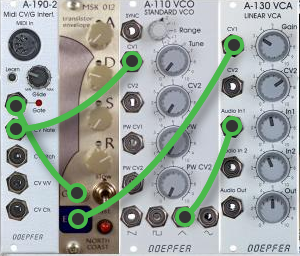
\includegraphics[scale=0.78]{patch1.png}\hspace*{\fill}\par} 

For a more deluxe version of the traditional subtractive patch, use separate
ADSR envelopes (both driven by the gate from the MIDI interface) to control
amplitude envelope and cutoff on the filter.  This example uses the built-in
VCA of the North Coast Leapfrog filter, but the same thing could easily be
done with a separate VCA module.

\nopagebreak\noindent
{\hspace*{\fill}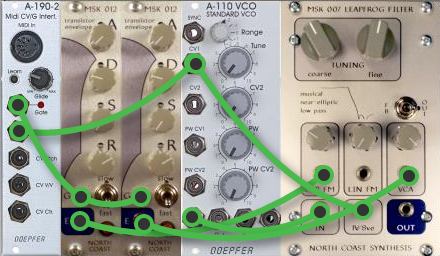
\includegraphics[scale=0.65]{patch2.png}\hspace*{\fill}\par} 

This is a sort of quick and dirty handclap patch; maybe also a finger-snap,
brushed drum, or a few other kinds of percussion, depending on the envelope
settings.  The key to all these kinds of sounds is getting the right
envelope shape, and it may be more complicated than just a basic ADSR.  Here
two MSK~012 modules have their outputs added by a DC mixer, with the result
controlling a VCA with white noise as the audio.  Normally the two ADSR
envelopes would be set on different time ranges, one ``fast'' and the other
``faster.'' One has minimum attack and a little bit of decay; the other has
a little bit of attack and minimum decay; both have zero sustain.  The sum
of the two envelopes gives a double peak typical of a handclap sound.

\nopagebreak\noindent
{\hspace*{\fill}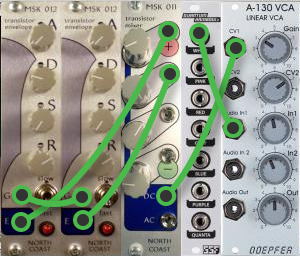
\includegraphics[scale=0.78]{patch3.png}\hspace*{\fill}\par} 

Chaining two envelopes, the first one set for slow attack and release and
maximum sustain level, creates a gate delay.  The second envelope won't
start until the attack of the first reaches about 2V, and won't end until
the first envelope's decay drops to about 1V.  If you want a well-behaved
gate voltage for something else, the second envelope can be set to very fast
range, minimum attack and release, maximum sustain level, to get a nice
square-sided 8V pulse output.  But if you just want a delayed envelope, the
second ADSR generator can be set to create the desired shape.

\nopagebreak\noindent
{\hspace*{\fill}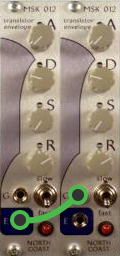
\includegraphics[scale=0.78]{patch4.png}\hspace*{\fill}\par} 

\pagebreak

Because of the Schmitt trigger on the gate input, which activates on voltage
levels without requiring a sharp edge, the MSK~012 can be used to condition
signals for other modules with pickier inputs.  Here, the Z3000's built-in
frequency counter/tuner requires sharp-edged signals and cannot get a
reading on the smooth waveform of the Hikari Sine.  Feeding the sine wave
through an MSK~012 (fastest speed range, minimum attack and release times,
maximum sustain level) converts it into a 0-8V pulse wave, which the Z3000
can reliably measure.

\nopagebreak\noindent
{\hspace*{\fill}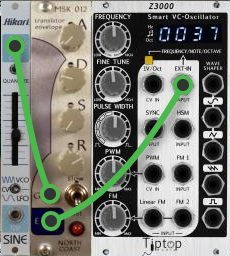
\includegraphics[scale=0.78]{patch5.png}\hspace*{\fill}\par} 
